% Official CVPR 2027 author kit, review mode.
\documentclass[10pt,twocolumn,letterpaper]{article}
\usepackage[review]{cvpr}
\usepackage{amsmath,amssymb}
\usepackage{booktabs,multirow}
\usepackage{graphicx}
\usepackage{microtype}
\usepackage{siunitx}
\usepackage{algorithm}
\usepackage{algpseudocode}
\usepackage{enumitem}
\usepackage{xspace}
\usepackage{balance}
\newcommand{\method}{PV-SRA-3DGS\xspace}
\newcommand{\ours}{pressure-triggered preservation\xspace}
\DeclareMathOperator*{\argmax}{arg\,max}
\setlength{\abovecaptionskip}{3pt}
\setlength{\belowcaptionskip}{-2pt}
\setlist[itemize]{leftmargin=*,nosep}

\definecolor{cvprblue}{rgb}{0.21,0.49,0.74}
\usepackage[pagebackref,breaklinks,colorlinks,allcolors=cvprblue]{hyperref}
\def\confName{CVPR}
\def\confYear{2027}

\title{Peak-VRAM-Constrained Spatial Resource Allocation with\\Pressure-Triggered Preservation for 3D Gaussian Splatting}
\author{Anonymous CVPR submission}

\begin{document}
\maketitle
\begin{abstract}
Training 3D Gaussian Splatting (3DGS) on memory-limited GPUs is difficult because densification changes both persistent model state and transient optimizer memory, while aggressive pruning can remove newly useful primitives before they accumulate sufficient evidence. We present \method, a spatial resource-allocation framework that regulates clone and split mutations under a calibrated peak-VRAM budget. Its central mechanism is pressure-triggered preservation: low-opacity or low-utility Gaussians remain eligible for optimization while measured allocator headroom is sufficient and are evicted only when admission requires space. A dynamic inflow governor varies mutation admission between 5K and 15K candidates, and a gain-per-byte allocator selects feasible clone and split operations using calibrated affine costs. On an 8,150.56-MiB RTX 5060 Laptop GPU, we evaluate 24 physical 30K-step runs over Bonsai, Garden, and Flowers. In a seed-0 2x2 factorial study, preservation has a $+10.14$ dB PSNR main effect; the inflow-by-lifecycle interaction is $-3.41$ dB. Across three Bonsai seeds, preservation improves the memory-bounded baseline by $11.09\pm2.34$ dB (paired $t(2)=8.21$, $p=0.0145$), but the small sample precludes broad inferential claims. Single-seed gains are $+6.25$ dB on Garden and $+2.94$ dB on Flowers. All 24 runs complete without observed OOM; sampled physical peaks range from 6,906 to 7,656 MiB. These results establish empirical boundedness under the tested workload, not a hardware-level memory guarantee.
\end{abstract}

\section{Introduction}
Neural radiance fields made photorealistic novel-view synthesis possible, but their volumetric evaluation is expensive~\cite{mildenhall2020nerf,barron2021mipnerf,muller2022instant,chen2022tensorf}. 3D Gaussian Splatting (3DGS) replaces repeated network queries with an explicit set of anisotropic Gaussians and a differentiable tile rasterizer, yielding high quality and real-time rendering~\cite{kerbl2023gaussians}. Its efficiency at inference, however, does not make training memory-free. Adaptive density control repeatedly clones and splits primitives; parameters, gradients, optimizer moments, temporary concatenations, and rasterization buffers coexist during mutation.

This distinction matters on consumer GPUs. A fixed Gaussian-count cap ignores the different transient costs of cloning and splitting and the current state of the caching allocator. Conversely, frequent opacity or utility pruning can be counterproductive: a new Gaussian often begins with weak opacity and incomplete view support, so a policy that applies hygiene eviction at every density-control cycle can remove it before optimization establishes its value. We call this the \emph{over-pruning dilemma}: freeing memory early may prevent the representation from reaching a useful spatial allocation.

We study the problem under an explicit peak-memory operating envelope rather than post-training model compression. Figure~\ref{fig:framework} summarizes \method. The system estimates current headroom from allocated and reserved CUDA memory, adds a non-PyTorch allowance, predicts affine clone/split costs, and admits a feasible mutation batch. Within that batch, a greedy gain-per-byte allocator prioritizes spatial demand. The main empirical finding is that the lifecycle policy dominates the inflow schedule: retaining low-scored Gaussians when headroom is sufficient, and pruning them only under admission pressure, produces much higher reconstruction quality than unconditional hygiene pruning in the evaluated implementation.

\begin{figure*}[t]
  \centering
  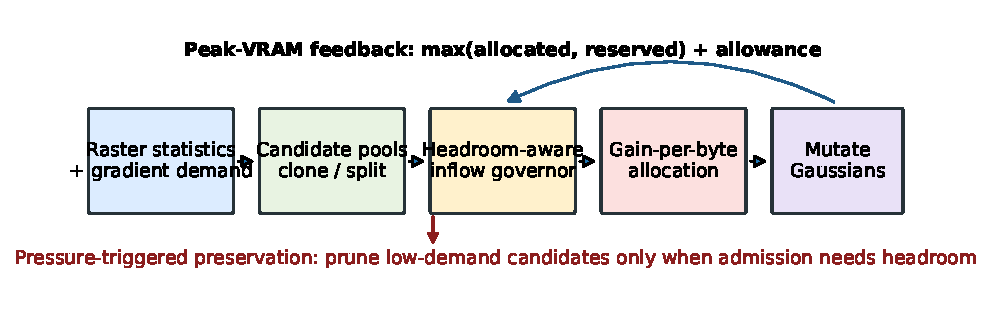
\includegraphics[width=\textwidth]{figures/fig1_framework.pdf}
  \caption{\method closes the loop between raster-derived spatial demand and allocator headroom. Pressure-triggered preservation is an admission-dependent lifecycle rule, not a post-training compression stage.}
  \label{fig:framework}
\end{figure*}

Our contributions are:
\begin{itemize}
  \item a peak-VRAM-aware mutation controller with calibrated affine clone/split costs and a dynamic 5K--15K inflow policy;
  \item a pressure-triggered preservation lifecycle that couples eviction to actual headroom demand, avoiding eager removal of under-optimized primitives;
  \item a complete 2x2 inflow-by-lifecycle ablation, three-seed paired validation on Bonsai, and single-seed evaluation on two additional Mip-NeRF 360 scenes;
  \item an evidence-traceable memory study that separates controller footprint from sampled whole-device VRAM and limits the claim to empirical boundedness.
\end{itemize}

\section{Related Work}
\paragraph{Radiance fields and explicit splatting.}
NeRF~\cite{mildenhall2020nerf}, mip-NeRF~\cite{barron2021mipnerf}, mip-NeRF 360~\cite{barron2022mipnerf360}, TensoRF~\cite{chen2022tensorf}, Plenoxels~\cite{fridovichkeil2022plenoxels}, and Instant-NGP~\cite{muller2022instant} progressively improve quality and training or rendering efficiency. 3DGS~\cite{kerbl2023gaussians} instead optimizes explicit anisotropic Gaussians and adapts their population through cloning, splitting, opacity removal, and scale-based pruning. Mip-Splatting addresses aliasing across sampling rates~\cite{yu2024mipsplatting}; Pixel-GS and Mini-Splatting revise density control and primitive placement~\cite{cheng2024pixelgs,fang2024minisplatting}. These methods motivate better population management but do not directly regulate transient mutation batches against a live peak-VRAM envelope.

\paragraph{Compact and efficient Gaussian representations.}
LightGaussian, Compact 3D Gaussian Representation, EAGLES, compressed 3DGS, and RDO-Gaussian reduce storage through pruning, masks, quantization, or adaptive attributes~\cite{fan2024lightgaussian,lee2024compact,girish2024eagles,niedermayr2024compressed,wang2024rdo}. Scaffold-GS structures Gaussians with anchors~\cite{lu2024scaffold}; Taming 3DGS targets high-resolution scenes~\cite{mallick2024taming}. More recent pruning work uses uncertainty, probabilistic masks, or alternating optimization~\cite{hanson2025pup,liu2025maskgaussian,zhang2025gaussianspa}; Speedy-Splat and FastGS target sparse computation and training speed~\cite{hanson2025speedysplat,ren2026fastgs}; LOD-GS introduces scalable levels of detail~\cite{shen2025lodgs}. Their primary objective is usually final representation size, rendering rate, or training speed. Our focus is complementary: safe and productive \emph{training-time inflow} under a measured memory budget.

\begin{table}[t]
\centering\scriptsize
\caption{Positioning relative to representative efficiency work. ``Peak feedback'' denotes live allocator-state control during densification.}
\label{tab:related}
\resizebox{\columnwidth}{!}{%
\begin{tabular}{lccc}
\toprule
Method family & Compact output & Peak feedback & Lifecycle\rule{0pt}{1.7ex} \\
\midrule
Light/Compact/RDO-GS & \checkmark & -- & prune/compress \\
PUP/Mask/GaussianSpa & \checkmark & -- & learned/optimized \\
Speedy-Splat/FastGS & partial & -- & efficiency-driven \\
\method & incidental & \checkmark & pressure-triggered \\
\bottomrule
\end{tabular}
}
\end{table}

\paragraph{Memory-aware allocation.}
Our allocator uses the classical gain-per-cost intuition of greedy knapsack selection~\cite{martello1990knapsack} but applies it to heterogeneous 3DGS mutation costs. Because PyTorch uses a caching allocator~\cite{paszke2019pytorch}, reserved memory, live allocation, fixed operation overhead, and external device use must not be conflated. We therefore report both an internal conservative footprint and asynchronously sampled total device VRAM.

\section{Method}
\subsection{Problem Formulation}
At iteration $t$, the scene is a set $\mathcal{G}_t=\{G_i\}_{i=1}^{N_t}$ of anisotropic Gaussians with position, scale, rotation, opacity, and spherical-harmonic appearance. Standard alpha compositing renders a pixel by depth-ordering contributing Gaussians and computing
\begin{equation}
  C(\mathbf{p})=\sum_{i} T_i\alpha_i c_i,\qquad
  T_i=\prod_{j<i}(1-\alpha_j).
\end{equation}
Training minimizes the implementation's photometric objective, $\mathcal{L}=0.8\mathcal{L}_1+0.2(1-\mathrm{SSIM})$, while density control proposes clone and split operations. Let $A_t$ and $R_t$ be PyTorch allocated and reserved memory, $B_{\rm hard}$ the controller limit, $B_{\rm safe}$ the safety margin, and $B_{\rm np}$ a non-PyTorch allowance. The controller's available headroom is
\begin{equation}
H_t=\max\!\left(0,B_{\rm hard}-B_{\rm safe}-[\max(A_t,R_t)+B_{\rm np}]\right).
\label{eq:headroom}
\end{equation}
This is a process-level control quantity; it is not equal to whole-device VRAM.

For SH degree three, each Gaussian has 59 FP32 values (236 B). The training model counts parameters, gradients, and two Adam moments, giving $c_p=944$ B/Gaussian. Profiling fits affine transient costs
\begin{align}
M_{\rm clone}(n)&=o_c+n\mu_c c_p, & \mu_c&=1.204584,\\
M_{\rm split}(n)&=o_s+n\mu_s c_p, & \mu_s&=2.573835,
\end{align}
where $o_c=60{,}231{,}489$ B and $o_s=124{,}401{,}559$ B. The held-out largest-batch combined MAPE is 3.57\%; consequently, the model is an empirical predictor rather than a proof of physical boundedness.

\subsection{Headroom-Constrained Inflow and Allocation}
Density control forms clone and split candidate sets from accumulated view-space gradients and scale. With $C_{\min}=5{,}000$, $C_{\max}=15{,}000$, and target headroom $H^*=1{,}024$ MiB, the dynamic item cap is
\begin{equation}
C_t=\min\!\left(C_{\rm mem},
C_{\min}+\left\lfloor\alpha_t(C_{\max}-C_{\min})\right\rfloor\right),
\end{equation}
where $\alpha_t=0$ when $H_t\le H^*$ and otherwise $\min(1,(H_t-H^*)/H^*)$. $C_{\rm mem}$ is the number of worst-case-cost items that fit after fixed overhead and padding. The static ablation instead uses $\min(C_{\min},C_{\rm mem})$.

Each candidate $i$ has compensated spatial demand $d_i$ and operation cost $c_i$. After reserving a feasible split share up to $\kappa=0.40$ when the byte budget permits, the allocator sorts remaining candidates by
\begin{equation}
\lambda_i=d_i/c_i
\end{equation}
and greedily admits operations until either the transient-byte or item cap is reached. If the requested batch does not fit, the controller first prunes lowest-demand candidates; if this cannot create enough headroom, it shrinks the batch by binary search.

\subsection{Pressure-Triggered Preservation}
The evaluated lifecycle factor compares two operational policies. \emph{Eager hygiene} applies opacity and size eviction at every 100-step density-control cycle independently of admission. The implementation includes age and post-reset exceptions in this path. \emph{Pressure-triggered preservation}, used by the best configuration, instead places low-opacity and bottom-utility Gaussians in the removable pool but executes removal only for \texttt{PRUNE-FIRST} or \texttt{SHRINK-AND-PRUNE-FIRST}. Thus an under-optimized Gaussian survives while headroom suffices and can continue receiving gradient updates (Fig.~\ref{fig:lifecycle}).

Crucially, the winning preservation configuration does \emph{not} test an explicit maturity threshold: although the codebase stores a birth iteration and exposes $\tau_{\rm age}=500$, that test belongs to the eager-hygiene branch and is not consulted by the preservation cells. We therefore treat preservation as admission-coupled deferred eviction, not as a proven developmental-age model.

\begin{figure}[t]
  \centering
  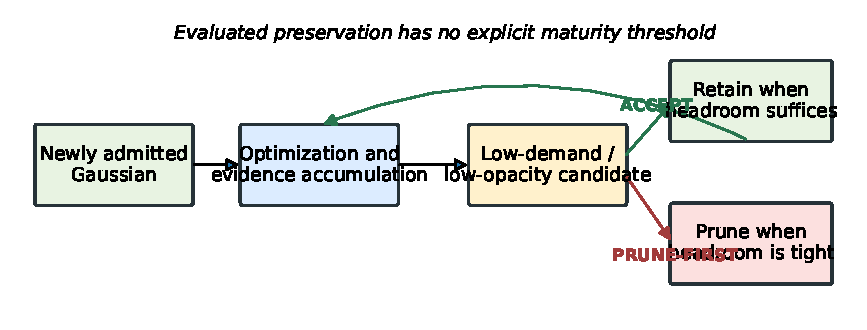
\includegraphics[width=\columnwidth]{figures/fig2_lifecycle.pdf}
  \caption{Operational lifecycle in the evaluated preservation configuration. Retention is conditional on headroom, with no explicit age threshold.}
  \label{fig:lifecycle}
\end{figure}

\begin{algorithm}[t]
\caption{Peak-VRAM-constrained mutation cycle}
\label{alg:method}
\small
\begin{algorithmic}[1]
\Require $\mathcal{G}_t$, clone/split masks, demand $d$, memory state
\State compute $H_t$ by Eq.~\eqref{eq:headroom} and affine costs
\State compute static or dynamic inflow cap $C_t$
\If{requested transient cost exceeds $H_t$}
  \State prune lowest-demand removable Gaussians
  \State recompute headroom and shrink batch if required
\EndIf
\State rank feasible candidates by $d_i/c_i$
\State enforce population cap and feasible split share $\kappa$
\State execute selected clones, then selected splits
\State log internal memory, admissions, rejections, and population
\end{algorithmic}
\end{algorithm}

\subsection{Complexity and Memory}
With $N$ active Gaussians and $K$ mutation candidates, demand and masks require $O(N)$ work and storage; sorting costs $O(K\log K)$ time and $O(K)$ temporary storage. Admission arithmetic and the 32-step shrink search are $O(1)$ in $N$. The base model stores an 8-B birth-iteration integer per Gaussian for the alternate eager-hygiene path, but pressure-triggered preservation itself adds no maturity metadata. These bounds exclude rasterization, whose tile lists depend on image content and view geometry.

\begin{table}[t]
\centering\scriptsize
\caption{Controller complexity beyond differentiable rendering.}
\label{tab:complexity}
\begin{tabular}{lcc}
\toprule
Component & Time & Auxiliary space\\
\midrule
Demand/masks & $O(N)$ & $O(N)$\\
Candidate sorting & $O(K\log K)$ & $O(K)$\\
Admission/shrink & $O(1)$ & $O(1)$\\
Birth index (optional path) & -- & 8 B/Gaussian\\
\bottomrule
\end{tabular}
\end{table}

\section{Experimental Setup}
\paragraph{Hardware and software.}
All reported training runs used one NVIDIA GeForce RTX 5060 Laptop GPU with 8,150.56 MiB physical VRAM under Windows 11/WDDM, driver 573.24, Python 3.12.10, PyTorch 2.11.0+cu128, and CUDA runtime 12.8. The internal controller used $B_{\rm hard}=6{,}144$ MiB, $B_{\rm safe}=512$ MiB, and $B_{\rm np}=256$ MiB. A separate thread queried \texttt{nvidia-smi} every 1.5 s; we call the maximum sample ``peak physical VRAM.'' Because spikes between samples can be missed, it is a sampled peak rather than continuous instrumentation.

\paragraph{Data and protocol.}
We use Bonsai, Garden, and Flowers from Mip-NeRF 360~\cite{barron2022mipnerf360}, loaded from \texttt{images\_4}. The standard LLFF rule holds out cameras with sorted index $i\bmod 8=0$, producing 255/37, 161/24, and 151/22 train/test views, respectively. Every run trains for 30,000 iterations; density control operates every 100 steps from iterations 500 to 15,000. Evaluation averages PSNR, SSIM~\cite{wang2004ssim}, and VGG-LPIPS~\cite{zhang2018lpips} over all held-out images. Final populations come from PLY vertex headers. Seeds 0, 1, and 2 are used for the paired Bonsai study; Garden and Flowers use seed 0 only.

\begin{table}[t]
\centering\scriptsize
\caption{2x2 factorial configurations. ``Preserve'' is the admission-coupled lifecycle described in Sec.~3.3.}
\label{tab:configs}
\resizebox{\columnwidth}{!}{%
\begin{tabular}{lcc}
\toprule
Configuration & Inflow & Lifecycle\\
\midrule
Baseline V4 (A1\_V4\_P1) & Dynamic 5K--15K & Eager hygiene\\
ABL-DI & Static 5K & Eager hygiene\\
ABL-DI-HP & Static 5K & Preserve\\
ABL-HP (ours) & Dynamic 5K--15K & Preserve\\
\bottomrule
\end{tabular}
}
\end{table}

\paragraph{Comparisons and statistics.}
The 2x2 factorial grid holds scene, seed, iteration count, learning schedule, population ceiling (1.15M), allocator, and memory settings fixed. It isolates inflow and lifecycle on Bonsai seed 0. We additionally compare to a vanilla 3DGS reference on Bonsai only; no vanilla reference was run on Garden or Flowers. For paired seed differences we report sample mean, sample standard deviation, a two-sided paired Student $t$ test, 95\% $t$ confidence interval, and Cohen's $d_z$. With $n=3$, the normality assumption cannot be meaningfully assessed; the exact two-sided sign test for three positive differences is only $p=0.25$.

\paragraph{Reproducibility.}
Python, NumPy, and PyTorch RNGs receive the recorded seed. Raw evaluation JSON, final PLY, checkpoints, command-line flags, telemetry, environment, exit status, and peak device sample are retained for each run. The validation script reads these artifacts directly and checks all 24 entries against the canonical registry; no new GPU experiment is used in this paper-writing pass.

\section{Results}
\subsection{Main and Multi-Seed Results}
Table~\ref{tab:seeds} shows every paired Bonsai run. Pressure-triggered preservation raises mean PSNR from $20.7455$ to $31.8305$ dB and reduces variability. The paired gain is $11.0850\pm2.3383$ dB, with $t(2)=8.2110$, $p=0.01451$, $d_z=4.7406$, and 95\% CI $[5.28,16.89]$ dB. These parametric statistics describe this three-seed sample; they are not evidence of dataset-wide significance. Mean SSIM changes from $0.6901$ to $0.9428$, and LPIPS from $0.4783$ to $0.1667$.

\begin{table*}[t]
\centering\scriptsize
\caption{Paired Bonsai results. Peak is sampled whole-device VRAM. Mean $\pm$ SD uses the three independent seeds.}
\label{tab:seeds}
\begin{tabular}{lccccccc}
\toprule
Policy & Seed & PSNR $\uparrow$ & SSIM $\uparrow$ & LPIPS $\downarrow$ & Gaussians & Peak (MiB) & Time (s)\\
\midrule
Eager hygiene & 0 & 22.8399 & .7430 & .3975 & 1,106,240 & 7,414 & 1,428.8\\
& 1 & 19.2472 & .6557 & .5359 & 570,389 & 7,513 & 1,014.7\\
& 2 & 20.1494 & .6715 & .5015 & 664,327 & 7,256 & 1,099.8\\
& mean $\pm$ SD & $20.7455\pm1.8690$ & $.6901\pm.0465$ & $.4783\pm.0721$ & $780,319\pm286,137$ & $7,394\pm130$ & --\\
\midrule
Preservation & 0 & 31.2776 & .9376 & .1737 & 705,392 & 7,444 & 1,608.1\\
& 1 & 32.1158 & .9447 & .1645 & 724,843 & 7,364 & 1,974.8\\
& 2 & 32.0981 & .9460 & .1619 & 783,091 & 7,205 & 2,255.7\\
& mean $\pm$ SD & $\mathbf{31.8305\pm.4789}$ & $\mathbf{.9428\pm.0045}$ & $\mathbf{.1667\pm.0062}$ & $737,775\pm40,432$ & $7,338\pm122$ & --\\
\bottomrule
\end{tabular}
\end{table*}

On Bonsai, the vanilla reference obtains 29.5857 dB with 1,235,390 Gaussians and a 7,656-MiB peak. The preservation mean is 2.2448 dB higher with 40.28\% fewer Gaussians. This is a scene-specific observation, not a general superiority claim. Figure~\ref{fig:qmem} further shows why population cannot substitute for measured memory: configurations with very different counts occupy overlapping whole-device peak ranges.

\begin{figure}[t]
\centering
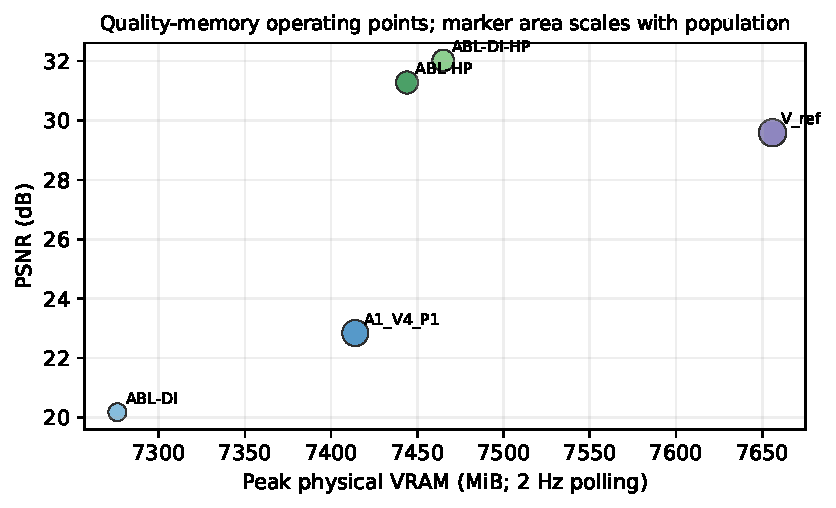
\includegraphics[width=\columnwidth]{figures/fig4_quality_memory.pdf}
\caption{Bonsai seed-0 operating points. Marker area scales with final Gaussian count; whole-device peak VRAM is not monotonic in population.}
\label{fig:qmem}
\end{figure}

\subsection{Factorial Ablation}
Table~\ref{tab:factorial} and Fig.~\ref{fig:factorial} give the complete seed-0 factorial grid. Averaging over inflow policies, preservation contributes $+10.1432$ dB PSNR, $+0.2179$ SSIM, and $-0.2600$ LPIPS. Averaging over lifecycles, dynamic inflow contributes $+0.9605$ dB. The interaction is substantial: dynamic rather than static inflow changes PSNR by $+2.6660$ dB under eager hygiene but by $-0.7451$ dB under preservation, a difference-in-differences of $-3.4111$ dB. Hence the inflow main effect should not be interpreted independently of lifecycle.

\begin{table*}[t]
\centering\scriptsize
\caption{Full 2x2 factorial ablation on Bonsai, seed 0. Each cell is one physical run.}
\label{tab:factorial}
\begin{tabular}{llccccc}
\toprule
Inflow & Lifecycle & PSNR $\uparrow$ & SSIM $\uparrow$ & LPIPS $\downarrow$ & Gaussians & Peak MiB\\
\midrule
Static 5K & Eager hygiene & 20.1739 & .7044 & .4691 & 358,651 & 7,276\\
Dynamic 5K--15K & Eager hygiene & 22.8399 & .7430 & .3975 & 1,106,240 & 7,414\\
Static 5K & Preserve & \textbf{32.0227} & \textbf{.9456} & \textbf{.1618} & 653,344 & 7,465\\
Dynamic 5K--15K & Preserve & 31.2776 & .9376 & .1737 & 705,392 & 7,444\\
\bottomrule
\end{tabular}
\end{table*}

\begin{figure}[t]
\centering
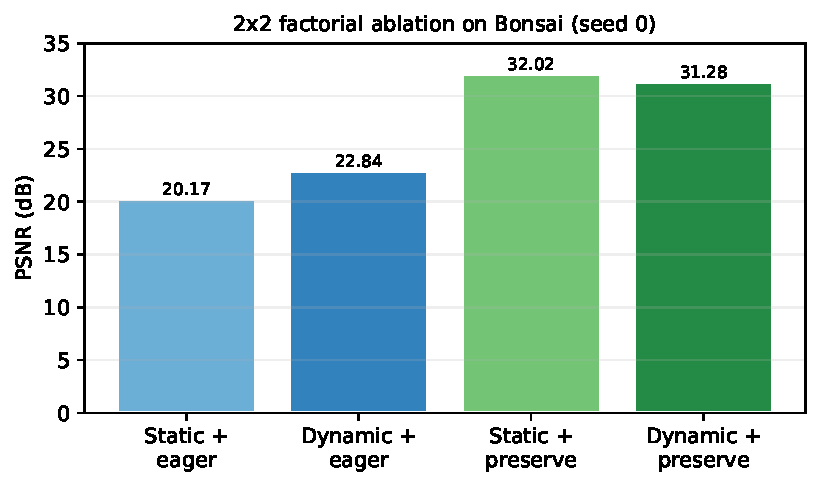
\includegraphics[width=\columnwidth]{figures/fig3_factorial.pdf}
\caption{Lifecycle dominates the seed-0 factorial result; dynamic inflow helps only under eager hygiene in this grid.}
\label{fig:factorial}
\end{figure}

\subsection{Cross-Scene Evaluation}
Preservation improves all three tested scenes relative to the matching memory-bounded baseline (Table~\ref{tab:crossscene}). Garden gains 6.2543 dB, $+0.3608$ SSIM, and $-0.3645$ LPIPS; Flowers gains 2.9422 dB, $+0.1793$ SSIM, and $-0.1846$ LPIPS. These are paired seed-0 observations. Only Bonsai has multi-seed replication.

\begin{table}[t]
\centering\scriptsize
\caption{Cross-scene seed-0 results (baseline $\rightarrow$ preservation).}
\label{tab:crossscene}
\begin{tabular}{lccc}
\toprule
Scene & PSNR & SSIM & LPIPS\\
\midrule
Bonsai & $22.84\!\rightarrow\!31.28$ & $.743\!\rightarrow\!.938$ & $.397\!\rightarrow\!.174$\\
Garden & $18.67\!\rightarrow\!24.93$ & $.385\!\rightarrow\!.746$ & $.674\!\rightarrow\!.310$\\
Flowers & $17.36\!\rightarrow\!20.30$ & $.338\!\rightarrow\!.517$ & $.651\!\rightarrow\!.466$\\
\bottomrule
\end{tabular}
\end{table}

\begin{figure}[t]
\centering
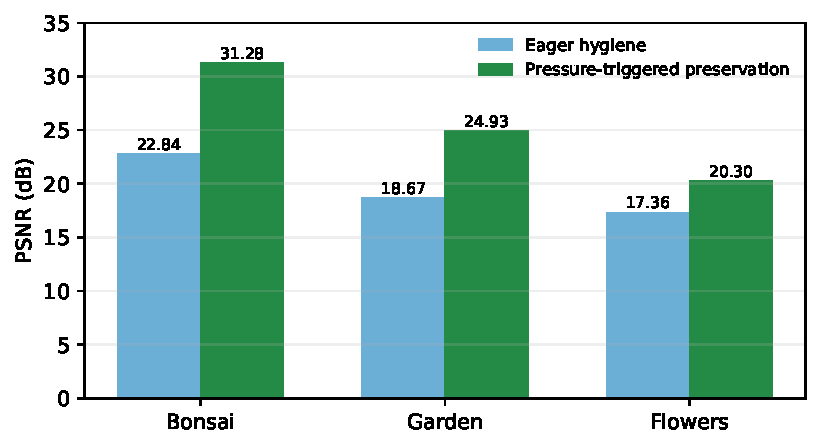
\includegraphics[width=\columnwidth]{figures/fig5_cross_scene.pdf}
\caption{Seed-0 PSNR across the three evaluated Mip-NeRF 360 scenes.}
\label{fig:crossscene}
\end{figure}

\subsection{Memory and Quality--Memory Trade-off}
All 24 audited physical runs complete with exit code zero and no recorded OOM. Sampled peaks span 6,906--7,656 MiB, leaving at least 494.56 MiB relative to the reported 8,150.56-MiB capacity. For the proposed seed-0 runs, Bonsai, Garden, and Flowers peak at 7,444, 7,570, and 7,288 MiB, respectively. Garden preservation increases population from 336,391 to 580,115 while reducing the sampled peak by 86 MiB; Flowers preservation reduces population from 707,777 to 426,905 while increasing the peak by 346 MiB. External WDDM use, rasterization buffers, timing, and allocator fragmentation therefore dominate any simple count-to-physical-memory relation.

\begin{table}[t]
\centering\scriptsize
\caption{Memory efficiency of seed-0 preservation runs. Headroom is capacity minus sampled peak.}
\label{tab:memory}
\begin{tabular}{lrrr}
\toprule
Scene & Gaussians & Peak MiB & Headroom MiB\\
\midrule
Bonsai & 705,392 & 7,444 & 706.56\\
Garden & 580,115 & 7,570 & 580.56\\
Flowers & 426,905 & 7,288 & 862.56\\
\bottomrule
\end{tabular}
\end{table}

The internal telemetry trace (supplementary Fig.~S1) remains below the controller's 5,632-MiB effective budget in the shown runs. This does not imply that total physical VRAM follows the same curve; the quantities have different scopes.

\section{Discussion}
\paragraph{Why preservation helps.}
The factorial evidence supports a lifecycle explanation, but not a microscopic causal proof. Eager hygiene evaluates opacity every density-control cycle. A recently admitted primitive can therefore be removed while its opacity and view support are still weak, even when memory is plentiful. Pressure-triggered preservation converts this unconditional decision into a resource-contingent one. The retained population has more opportunities to redistribute spatial support, which is consistent with the large quality gains and lower seed-to-seed variance. Direct per-Gaussian lineage experiments would be required to prove that maturation, rather than another branch-level behavior, is the sole mechanism.

\paragraph{Inflow and lifecycle interact.}
Dynamic inflow partly compensates for eager pruning by injecting more candidates, explaining its $+2.67$ dB simple effect in that branch. Once preservation is active, static 5K is slightly better than dynamic inflow at seed 0. More admission is therefore not uniformly beneficial: candidate quality, optimization time, and retention jointly determine the final allocation. This interaction is the reason we do not present dynamic inflow as an independently validated quality improvement.

\paragraph{Fewer Gaussians can be better.}
Primitive count is a capacity measure, not a quality metric. The preservation mean exceeds the Bonsai vanilla reference with fewer Gaussians, plausibly because admission and retention place capacity where demand is higher. Yet whole-device VRAM is also not determined by count alone. Transient tensor concatenations, optimizer rebuilding, view-dependent rasterization lists, caching, and WDDM allocations can dominate a sampled physical peak.

\paragraph{Deployment implications.}
The controller is useful when a fixed training recipe must operate close to a consumer-GPU limit: it turns free headroom into a mutation budget and exposes explicit safety margins. It does not virtualize memory or intercept every rasterizer allocation. A deployment should therefore calibrate clone/split costs on its own software stack, reserve external headroom, and treat asynchronous device telemetry as diagnostic rather than preventive.

\section{Limitations}
Our evidence is intentionally narrow. All training uses a single RTX 5060 Laptop GPU and one Windows/WDDM stack; calibration and external-memory behavior may change on datacenter GPUs, Linux, different PyTorch allocators, or other resolutions. Only three Mip-NeRF 360 scenes are tested. Bonsai has three paired seeds, but $n=3$ gives only two degrees of freedom and makes the $t$ result sensitive to distributional assumptions; Garden and Flowers have one seed each. The exact sign test is not significant at 0.05.

Peak physical VRAM is sampled every 1.5 s, so sub-interval transients may be missed. The controller observes PyTorch allocation and reservation plus a fixed allowance, not every driver or rasterizer allocation; zero OOM in 24 runs is empirical boundedness, not a formal guarantee. The affine cost model's 3.57\% held-out combined MAPE also leaves modeling error.

The vanilla reference exists only for Bonsai, and the repository does not contain matched physical baselines for recent compression and pruning systems~\cite{hanson2025pup,liu2025maskgaussian,zhang2025gaussianspa}. We therefore compare those works conceptually, not numerically. Finally, the winning branch is an admission-coupled deferred-eviction implementation historically named \texttt{legacy\_as\_is}; it does not use the codebase's explicit age threshold. Broader benchmarks and per-Gaussian lineage logging are needed to separate preservation duration, opacity dynamics, and utility estimation.

\section{Conclusion}
We studied 3DGS training as spatial resource allocation under a peak-VRAM operating envelope. \method combines calibrated affine mutation costs, headroom-aware inflow, gain-per-byte selection, and pressure-triggered preservation. Across the evaluated configurations, lifecycle choice is the dominant factor: delaying eviction until admission needs space substantially improves reconstruction quality, while the benefit of dynamic inflow depends on that lifecycle. Twenty-four physical runs finish without observed OOM on an 8-GB laptop GPU, but the evidence supports only empirical boundedness. Future work should replicate the factorial design across more scenes, seeds, GPUs, and recent baselines; record high-frequency device telemetry; and test explicit, lineage-aware maturity policies against the simpler pressure trigger identified here.


\clearpage
{\small
\bibliographystyle{ieeenat_fullname}
\bibliography{references}
}

\section*{LLM Usage Statement}
An OpenAI Codex language model assisted with manuscript drafting, code-based figure generation, and consistency checking. The authors are responsible for the research design, source code, experimental evidence, claims, and final text. No model-generated experimental result or citation is reported without verification against the repository artifacts or a primary publication source.
\end{document}
